\chapter{Geometry reconstruction using constrained nonlinear optimization}\label{ch:optimization}

\vspace{-1.5 em}
\begin{addmargin}[-0.5cm]{0cm}
  \minitoc
\end{addmargin}
\hrule
\vspace{1.5 em}

In the previous chapter, we saw that a lookup table approach could be used to perform geometry reconstruction using Coulomb explosion imaging. However, numerous drawbacks including the lookup table's exponential computational space complexity (severely limiting its scalability to larger molecules) and its inability to both provide precise reconstructions as well as distinguish between local and global minima leave much to be desired.

In this chapter, we will approach the task of geometry reconstruction as an optimization problem, allowing us to utilize the the much more sophisticated methods of constrained nonlinear optimization. Before we describe our reconstruction methods, it will be worthwhile to provide some background on the theoretical framework underpinning the optimization algorithms we utilize. We will then describe our implementation and use it to reconstruct the same molecular structures seen in the previous chapter, allowing for some comparison between methods and for some verification of the results. We will then further study the individual geometries recovered and the nature of the degenerate geometries seen in section \ref{sec:degenerateGeometries}. %, bringing to light some troubling issues regarding the problem of geometry reconstructing as well as highlighting its pathalogical nature.

\section{Mathematical optimization}
We will take a massively expedited tour of mathematical optimization with the aim of explaining the inner workings of the primal-dual interior point methods used for nonlinear constrained optimization in this chapter. To understand how these methods operate, we will need to introduce some important concepts in optimization, namely the duality principle, the Karush-Kuhn-Tucker (KKT) optimality conditions, and the general concept of a trust region. This is prefaced with a brief introduction to the subject.

No knowledge of mathematical optimization is required, however we will assume some background knowledge throughout this section, namely a familiarity with linear algebra, matrix algebra, vector calculus, and some elementary concepts in analysis. \citet{Boyd04} provides an excellent introduction to mathematical optimization, particularly convex optimization, and their freely-available textbook is accompanied by video lectures and lecture slides. We will follow their textbook for sections \ref{ssec:elementaryOptimization} to \ref{ssec:KKT}. Our problem is nonconvex, however, and so we also turn to \citet{Nocedal06} for sections \ref{ssec:trust} to \ref{ssec:interiorPoint}, who discuss the more advanced interior-point methods suitable for nonlinear constrained optimization with clarity.

\subsection{Elementary concepts} \label{ssec:elementaryOptimization}
The standard form of a (continuous) optimization problem is
\begin{align} \label{eq:op}
\mathrm{minimize}   \quad & f_0(x) \nonumber \\
\mathrm{subject\;to} \quad &
f_i(x) \leq 0, \; i \in \left\{1, \dots, m \right\}\\
& h_i(x) = 0, \; i \in \left\{1, \dots, p \right\} \nonumber
\end{align}
where $f_0(x): \mathbb{R}^n \rightarrow \mathbb{R}$ is the \emph{objective function} to be minimized over the variable $x \in \mathbb{R}^n$, $f_i(x) \leq 0$ are called the \emph{inequality constraints}, and $h_i(x) = 0$ are called the \emph{equality constraints}. The notation $f: A \rightarrow B$ denotes that $f$ is a \emph{function} (or \emph{mapping}) with \emph{domain} $A$, that is $A$ is its set of acceptable inputs, and \emph{codomain} $B$, that is $B$ is its set of acceptable outputs. We say that $f$ maps values from $A$ to $B$. $\mathbb{R}$ denotes the set of real numbers, and $\mathbb{R}^n$ denotes the $n$-dimensional real, or Eucliedian, vector space, that is the set of $n$-dimensional vectors with real components. The notation $x \in S$ denotes that $x$ is an element of the set $S$.

We denote the domain of the optimization problem \eqref{eq:op}by
\begin{equation}
\mathcal{D} = \bigcap_{i=1}^m \operatorname{dom} f_i \cap \bigcap_{i=1}^p \operatorname{dom} h_i \neq \emptyset
\end{equation}
and assume it is nonempty. The $\cap$ operator denotes the intersection operation and the $\emptyset$ denotes the empty set, both from set theory \citep{Halmos17}. The operator $\operatorname{dom} f$ denotes the domain of the function $f$. In effect, an optimization problem is only defined for regions where the objective function and all constraints are defined. An optimization problem is solved once an optimal solution, usually denoted $x^\star$, is found that minimizes the objective function $f_0(x)$ such that $f_0(x^\star) \le f_0(x)$ for all $x \in \mathcal{D}$.

Taking our geometry reconstruction problem as an example, we can describe our objective function as
\begin{equation} \label{eq:ourObjective}
f_0(x) = |p(x)-p_\textrm{measured}|^2
\end{equation}
where $p(x)$ is the momentum vectors produced following Coulomb explosion of a molecular with structure $x$, and the inequality constraints $f_i(x) \leq 0$ encapsulate the box constraints that limit the geometries recovered to physically reasonable values. For a triatomic molecule, $x = (r_{12}, r_{23}, \theta) \in \mathbb{R}^3$ may be used and $p(x) \in \mathbb{R}^9$ although it may be reduced to contain only $5$ or even $3$ nonzero components (see section \ref{sec:conventions}). For a general molecule with $N$ atoms, $x \in \mathbb{R}^{3N-6}$ and $p(x) \in \mathbb{R}^{3N-3}$ at most. We may wish to limit the reconstructed \ch{C-O} bond length to lie between \SIrange{100}{500}{\pico\m} in which case we would employ the inequality constraints $f_1(r_\mathrm{CO}) =  100 - r_\mathrm{CO} \le 0$ and $f_2(r_\mathrm{CO}) =  r_\mathrm{CO} - \SI{500}{\pico\m} \le 0$. Box constraints for the \ch{C-S} bond length and bond angle can be placed in a similar manner. Other contraints may be employed limiting, for example, the bond length ratio $r_\mathrm{CO}/r_\mathrm{CS}$ to lie between certain values pertaining to physically realizable geometries. We employ no equality constraints. Generally, $p(x)$ and $p_\textrm{measured}$ should be described in the same rotation convention otherwise they cannot be compared.

Optimization problems can be classified based on the nature of the objective function $f_0$ and the constraints $f_i$ and $h_j$, with each class having their own algorithms. Perhaps the simplest commonly encountered class is the class of \emph{linear programs} where the objective function and constraints are linear, that is $f_0, \dots, f_m, h_1, \dots, h_p$ all satisfy the linearity property
\begin{equation}
f_i(\alpha x + \beta y) = \alpha f_i(x) + \beta f_i(y)
\end{equation}
for all $x,y \in \mathbb{R}^n$ and $\alpha, \beta \in \mathbb{R}$. Although no analytical solution exists to solve an arbitrary linear program, efficient algorithms with computational run time $\mathcal{O}(n^2m)$ exist to find solutions, such as George Dantzig's simplex method.

\emph{Convex optimization problems} are a superset of linear programs and are characterized by having an objective function and constraint functions that all satisfy the convexity property
\begin{equation}
f_i(\alpha x + \beta y) \le \alpha f_i(x) + \beta f_i(y)
\end{equation}
for all $x,y \in \mathbb{R}^n$ and all $\alpha, \beta \in \mathbb{R}$ with $\alpha, \beta \ge 0$ and $\alpha + \beta = 1$. Commonly encountered convex function include the exponential function $e^x$ and the quadratic function $x^2$. In general, very mature and effective algorithms exist to solve convex optimization problems. If a problem can be transformed into convex form, then it becomes rather easy to solve, however this process can be very difficult and many tricks exist. Linear programs and the linear least squares problems are special case of convex optimization problems.

\emph{Nonlinear optimization} describes the class of problems where the objective or constraint functions are not linear, but not known to be convex. Unfortunately there are no effective algorithms for solving nonlinear problems in general but there are a number of approaches that may prove fruitful. These include the interior-point method we use and sequential quadratic programming. \citet{Sun15} provide an expository article on ``when nonconvex problem are not scary''.

Unfortunately the problem of geometry reconstruction falls under the category of nonlinear problems. While our objective function \eqref{eq:ourObjective} seems to mimic a least-squares minimization problem, it is certainly nonlinear in nature. There are two contributors to the nonlinear nature of our objective function. One is the existence of multiple solutions as evidenced by the existence of degenerate geometries we encountered in section \ref{sec:degenerateGeometries}. The other is the nonlinear nature of the objective function. A one-dimensional convex function must have a nonnegative second-derivative, and a multi-dimensional convex function must be twice-differentiable and have a positive semidefinite Hessian matrix over its domain \citep[p. 71]{Boyd04}. Nothing guarantees that this is true for our objective function.

Algorithms do exist for the solution of nonlinear least-squares problems such as NL2SOL \citep{Dennis81} and the Levenberg–Marquardt algorithm \citep{Pujol07}, however, modifying them to account for constraints usually introduces penalty functions and trust regions and they begin to appear quite similar to the interior-point methods described in section \ref{ssec:interiorPoint}. Examples include the open-source Interior Point OPTimizer (IPOPT) \citep{Branch99}.

% It is worth showing that not every least-squares minimization problem is a convex optimization problem.

\subsection{Duality}
In order to describe and understand the interior-point method we use, it is neccessary that we look at the concept of duality. Every optimization problem may be viewed from two different perspectives, that of the original, or \emph{primal}, problem and the \emph{dual} problem. Solving the dual problem provides a lower bound to the primal problem as we will show. Additional, by attempting to solve both problems at the same time, as interior-point methods do, an optimal solution may be found more efficiently.

We begin by defining the \emph{Langrangian} associated with the optimization problem \eqref{eq:op} as
\begin{equation}
L(x, \lambda, \nu) = f_0(x) + \sum_{i=1}^m \lambda_i f_i(x)
+ \sum_{i=1}^p \nu_i h_i(x)
\end{equation}
where $L: \mathbb{R}^m \times \mathbb{R}^p \rightarrow \mathbb{R}$ and $\operatorname{dom} L = \mathcal{D} \times \mathbb{R}^m \times \mathbb{R}^p$. $\lambda_i$ is the Langrange multiplier associated with the inequality constraint $f_i(x) \leq 0$ and $\nu_i$ is the Langrange multiplier associated with the equality constraint $h_i(x) = 0$. Together, $\lambda \in \mathbb{R}^m$, and $\nu \in \mathbb{R}^p$, are called the \emph{dual variables} or \emph{Langrange multiplier vectors}. The basic idea is that we're accounting for the constraint functions by adjusting the objective function to include a weighted sum of the constraint functions.

The \emph{Lagrange dual function} is defined as the minimum value of the Lagrangian $L$ over $x$
\begin{equation}
g(\lambda, \nu) = \inf_{x \in \mathcal{D}} L(x, \lambda, \nu)
= \inf_{x \in \mathcal{D}} \left[ f_0(x) + \sum_{i=1}^m \lambda_i f_i(x)
+ \sum_{i=1}^p \nu_i h_i(x) \right]
\end{equation}
where $g: \mathbb{R}^m \times \mathbb{R}^p \rightarrow \mathbb{R}$. The $\inf$ operator refers to the \emph{infimum} operator, which may also be called the  \emph{greatest lower bound} operator. An important property of the dual function is that it is concave even when the problem is not convex, as it is the pointwise infimum of a family of affine functions of $(\lambda, \nu)$.

\begin{theorem} \label{thm:lower}
  The Lagrange dual function yields a lower bound on the optimal value of the problem \eqref{eq:op} for $\lambda \succeq 0$ and any $\nu$.
\end{theorem}
\begin{proof}
  Denote the optimal value of the dual function by $p^\star$ and let $x'$ denote a feasible input of the Lagrangian, that is it satisfies the constraints $f_i(x') \le 0$ and $h_i(x') = 0$. Then for $\lambda \succeq 0$ and any $\nu$ we have that
  
  $$ \sum_{i=1}^m \lambda_i f_i(x') + \sum_{i=1}^p \lambda_i h_i(x') \le 0 $$
  so that
  $$ L(x',\lambda,\nu) = f_0(x') + \sum_{i=1}^m \lambda_i f_i(x') + \sum_{i=1}^p \lambda_i h_i(x') \le f_0(x') $$
  and
  $$ g(\lambda, \nu) = \inf_{x \in \mathcal{D}} L(x, \lambda, \nu) \le L(x', \lambda, \nu) \le f_0(x') $$
  which must hold for every feasible point $x'$ including the optimal solution $x^\star$ and thus
  $$ g(\lambda, \nu) \le p^\star = f_0(x^\star) $$ 
\end{proof}

As the lagrange dual function provides a lower bound on the optimal value $p^\star$ that depends on $(\lambda,\nu)$, we may be interested in finding the best lower bound. This leads to the \emph{Lagrange dual problem} associated with \eqref{eq:op} which can be stated as
\begin{align} \label{eq:dualop}
\mathrm{maximize}    \quad & g(\lambda, \nu) \nonumber \\
\mathrm{subject\;to} \quad & \lambda \succeq 0
\end{align}
and is always a convex problem as the dual function $g(\lambda, \nu)$ is always convex as mentioned when we introduced it. We can then talk about \emph{dual feasible} pairs $(\lambda,\nu)$ with $\lambda \succeq 0$ and $g(\lambda,\nu) > -\infty$, \emph{optimal Lagrange multipliers} or the \emph{dual optimal} pair $(\lambda^\star, \nu^\star)$, and the optimal value of the dual problem, denoted $d^\star$ . In some contexts involving both the dual problem \eqref{eq:dualop} and the original problem \eqref{eq:op}, the original problem is called the \emph{primal problem}.

If the optimal value of the dual problem $d^\star$ and of the primal problem $p^\star$ are equal, $d^\star = p^\star$, then we say that \emph{strong duality} holds and the \emph{optimal duality gap} is zero, $d^\star - p^\star = 0$. Otherwise $d^\star \le p^\star$ and we say that \emph{weak duality} holds.

\subsection{Optimality conditions} \label{ssec:KKT}
It will be quite useful to impose conditions on what makes a feasible solution an optimal solution for both the primal and dual problems. This will provide a means of checking whether a proposed solution is optimal, as every optimal solution must satisfy the optimality conditions. Denoting the optimal primal solution by $x^\star$ and the optimal value by $p^\star = f_0(x^\star)$, we already know that it must satisfy the inequality and equality constraints,
\begin{equation}
f_i(x^\star) \ge 0 \quad \mathrm{and} \quad h_i(x^\star) = 0
\end{equation}
giving us two optimality conditions so far. Denoting the dual optimal by $(\lambda^\star, \nu^\star)$ we would like for
\begin{equation}
\lambda_i^\star \ge 0
\end{equation}
so that the dual function provides a lower bound on $p^\star$ by theorem \ref{thm:lower}, giving us a third condition.

For the fourth condition, we look to the dual function and assume that strong duality holds, that is that $f_0(x^\star) = g(\lambda^\star, \nu^\star)$. Then we can write
\begin{align}
  f_0(x^\star) &= g(\lambda^\star, \nu^\star) \nonumber \\
  & = \inf_x \left[ f_0(x) + \sum_{i=1}^m \lambda_i^\star f_i(x) + \sum_{i=1}^p \nu_i^\star h_i(x) \right] \nonumber \\
  & \le f_0(x^\star)
    + \underbrace{\sum_{i=1}^m \lambda_i^\star f_i(x^\star)}_{\le 0}
    + \underbrace{\sum_{i=1}^p \nu_i^\star h_i(x^\star)}_{=0} \nonumber \\
  & \le f_0(x^\star)
\end{align}
where we invoked the definition of the dual function on the second line, and the third line follows from the fact that the Lagrangian evaluated at the optimal primal point $x^\star$ provides a lower bound. Then on the fourth line we realize that the equality constraint functions $h_i(x) = 0$ cause the third term to vanish, and we assumed that the Lagrange multipliers obeyed $\lambda_i^\star \ge 0$ while the inequality constraints satisfy $f_i(x) \le 0$ thus causing the second term to be nonpositive. However we require that equality hold on the fourth line as $f_0(x^\star)$ must equal itself. For equality to hold, we thus require that the second term vanish just like the third term,
\begin{equation}
  \sum_{i=1}^m \lambda_i f_i(x^\star) = 0
\end{equation}
however each term is nonpositive so we can recast this condition as
\begin{equation}
  \lambda_i f_i(x^\star) = 0, i = 1,2,\dots,m
\end{equation}
This provides a forth optimality condition, known as \emph{complementary slackness}.

For the fifth condition, we realize that a function's first-derivative must vanish at a minima or maxima. Since $x^\star$ minimizes the Lagrangian $L(x, \lambda^\star, \nu^\star)$ over $x$, its gradient must be zero at the minima or maximum $x^\star$, giving us
\begin{equation}
\nabla f_0(x^\star) + \sum_{i=1}^m \lambda_i^\star \nabla f_i(x^\star)
+ \sum_{i=1}^p \nu_i^\star \nabla h_i(x^\star) = 0
\end{equation}

Together, we can summarize the five conditions we obtained
\begin{align} \label{eq:kkt}
f_i(x^\star) & \geq 0, \; & i & \in {1,\dots,m} \nonumber \\
h_i(x^\star) & = 0, \; & i & \in {1,\dots,p} \nonumber \\
\lambda_i^\star & \geq 0, \; & i & \in {1,\dots,m} \\
\lambda_i^\star f_i(x^\star) & = 0, \; & i & \in {1,\dots,m} \nonumber \\
\nabla f_0(x^\star) + \sum_{i=1}^m \lambda_i^\star \nabla f_i(x^\star)
+ \sum_{i=1}^p \nu_i^\star \nabla h_i(x^\star) & = 0, \; & i & \in {1,\dots,m} \nonumber
\end{align}
which together are called the \emph{Karush-Kuhn-Tucker (KKT) conditions}. They are sometimes referred to as the first-order optimality conditions, as second-order conditions do exist \citep[\S 12.5]{Nocedal06}.

\subsection{Trust regions} \label{ssec:trust}
In general, when searching for an optimal solution an optimization algorithm begins from an initial guess $x_0$. Then successive guesses, or iterates, denoted by $x_k$ for the $k^\mathrm{th}$ guess or iterate are made with the aim of converging on the optimal solution $x^\star$.

Switching gears a little bit in this subsection, we'll look at a general strategy of solving optimization problem using the concept of a \emph{trust region} which may be used to determine the next iterate $x_{k+1}$. The idea is to create and solve an approximate optimization problem at each iterate $x_k$ with the hope that the approximation is easier to solve yet locally accurate enough to help locate the true optimal solution. The approximated is \emph{trusted} only so much, up to some radius or region boundary. A circular or spherical trust region may be used, but so can box and elliptical regions. If a sufficiently better iterate $x_{k+1}$ is not found within the trust region then the region may be shrunk in case the approximation becomes grossly invalid for points far way from the iterate $x_k$.

The approximation employed may be termed the \emph{model function} so that the approximate problem at iterate $x_k$ becomes
\begin{equation}
\operatorname{minimize}_p m_k(x_k + p)
\end{equation}
where $p$ is the candidate step so that $x_k + p$ lies within the trust region. A very popular model function takes the form of a quadratic approximation using the first two terms of a Taylor approximation of the objective function at the iterate point
\begin{equation}
  m_k(x_k + p) = f(x_k) + p^T \nabla f(x_k) + \frac{1}{2} p^T \nabla^2 f(x_k) p
\end{equation}
where $\nabla f(x_k)$ and $\nabla^2 f(x_k)$ are the gradient and Hessian of the objective function $f$ at the point $x_k$ \citep{More83}. A quadratic function is convex and thus such a convex ``subproblem'' that locally approximates the optimization problem can be solved efficiently.

Trust regions see a great deal of use in nonlinear optimization methods, and can be modified for constrained optimization. Beyond the choice of approximation and trust region type, choosing the region size and shape, the step size, and the method used to solve even the trust region subproblem are important. Another class of methods serving a similar purpose are line search methods where a direction is first chosen to search for the next iterate, so that the step size is chosen second. Line search methods are in a sense the dual of trust region methods, where the step size (trust region radius or boundary) is chosen first, then a direction is chosen.

\subsection{Primal-dual interior point methods} \label{ssec:interiorPoint}
Having discussed some important ideas and concepts from mathematical optimization theory, we can now begin to discuss the interior-point optimization method we rely on for geometry reconstruction in this chapter.

The idea behind an interior-point method is to modify the an original problem to take into account the constraint functions by modifying the objective function to penalize iterates that leave the feasible region (or break the constraints). As this may modify the optimal solution, the approximation is realxed as a local minimum is approached, so you are essentially solving a series of approximate optimization subproblems. A very popular approximation is to use a logarithmic barrier, that induces a penalty that approaches $\infty$ as you approach the constraint.

\begin{align}
\mathrm{minimize} \quad & f_\mu(x,s) = f(x) - \mu \sum_{i=1}^{m} \ln s_i \nonumber \\
\mathrm{subject\;to} \quad & g_i(x) + s_i = 0 \\
                           & h_i(x) = 0 \nonumber
\end{align}

Direct step
\begin{equation}
\begin{pmatrix}
  H   & 0        & J_h^T & J_g^T \\
  0   & S\Lambda & 0     & -S \\
  J_h & 0        & I     & 0 \\
  J_g & -S       & 0     & I
\end{pmatrix}
\begin{pmatrix}
  \Delta x  \\
  \Delta s  \\
  -\Delta y \\
  -\Delta \lambda \\
\end{pmatrix}
=
\begin{pmatrix}
\nabla f - J_h^T y - J_g^T \lambda  \\
S\Lambda - \mu e \\
h \\
g + s \\
\end{pmatrix}
\end{equation}
where $H$ is the Hessian of the Lagrangian of $f_\mu$
\begin{equation}
H = \nabla^2 f(x) + \sum_i \lambda_i \nabla^2 g_i(x) + \sum_j \lambda_j \nabla^2 h_j(x),
\end{equation}
$J_g$ and $J_h$ are the Jacobians of the constraint function $g$ and $h$ respectively, $S = \operatorname{diag}(s)$, $\Lambda = \operatorname{diag}(\lambda)$, $\lambda$ and $y$ are the Lagrange multipliers associated with the constraint functions $g$ and $h$ respectively, and $e$ is a vector of ones with the same size as $g$.


\subsection{Curse of dimensionality and possible solutions} \label{ssec:curse}
The curse of dimensionality, a term first introduced by \citet{Bellman57} when considering problems in dynamic optimization, refers to the exponential increase in volume when adding extra dimensions to Euclidean space \citep{Keogh10}. It manifests itself in two ways when tackling the geometry reconstruction problem for larger and larger molecules, as we need $3N-6$ parameters to describe the geometry of an molecule with $N \ge 3$ atoms. Firstly, the parameter space or phase space to be searched increases exponentially with $N$, and with this increase may come an increase in local minima, and possible an increase in the number of degenerate geometries. While we believe, anecdotally, that interior-point methods will still be feasible for polyatomic molecules with several atoms, convergence will definitely take longer and multiple runs may be required before finding a feasible geometry or any degenerate geometries, possibly necessitating the use of a supercomputer cluster.

The second manifestation, which seems more severe from preliminary investigations of reconstructing acetylene (\ch{C2H2}) molecular geometries, is the proliferation of saddle points in high-dimensional spaces, termed the \emph{saddle-point problem} as argued by \citet{Pascanu14} using evidence from statistical physics, random matrix theory, and neural network theory. Fortunately, this is a very active area of research due to the recent surge and revival of interest in artificial intelligence \citep{Bengio16,LeCun15} and the development of new algorithms may be helpful in reconstructing larger molecules. One recent example worth looking into for future improvements include the saddle-free Newton method proposed by \citet{Dauphin14} which uses second-curvature information to rapidly escape from high-dimensional saddle points.

One easy method of tackling this problem when attempting to reconstruct larger molecules is to fix certain parameters of the molecule's geometry, ones which may exhibit very low variability. An example may be the triple \ch{C+C} bond in acetylene.

\section{Implementation}
As mentioned in the previous section, there are many complications involved with implementing advanced optimization algorithms such as the interior-point method we wish to use, and so we turn to the readily-available and mature implemention in MATLAB's Optimization Toolbox in conjunction with the Global Optimization and Parallel Processing Toolboxes. In the spirit of open science and reproducibility, we strongly feel that we should have chosen an open-source implementation however this was not a consideration at the beginning of this project and the MATLAB implementation seems to be superior to most of the available alternatives we inspected, proprietary and open-source, and is well-documented and easy to use as opposed to specialized mathematical optimization software developed for research purposes. So we see the use of MATLAB as a neccessary evil at this point in time.

The concern behind relying on proprietary software is mainly to do with scientific reproducibility in computational studies \citep{Easterbrook14} for which \citet{Millman14} and \citet{Wilson14} provide excellent advice. MATLAB is popular enough and a standard piece of software in many fields that one may quite easily find a usable instance in an academic setting to run the code in appendix \ref{appx:code} and replicate the results presented here. However, in order to reproduce our results from scratch and verify their correctness, the optimization code would need to be inspected, which is impossible in this case due to the proprietary nature of MATLAB. This was not as big a concern with the lookup table as it did not rely on any MATLAB-specific library functions that do not have direct analogues in other programming environments.

For the implementation, the MATLAB Optimization Toolbox provides a general-purpose nonlinear programming solver, \texttt{fmincon}, that attempts to find the minimum of a constrained nonlinear multivariable objective function. Among the algorithms \texttt{fmincon} can employ is the interior-point method we described in the previous section. We use it to find geometries whose post-explosion momentum vectors most precisely match the measurements. We constrain the solution using \emph{box constraints} to ensure we recover triatomic geometries with the constraints that $\SI{100}{\pico\meter} \le r_\mathrm{CO}, r_\mathrm{CS} \le \SI{500}{\pico\meter}$ and $\SI{140}{\degree} \le \theta \le \SI{180}{\degree}$ for the \ch{OCS} molecule.

We use the objective function
\begin{equation}
\log_{10}|p(x)-p_\textrm{measured}|^2
\end{equation}
where $p(x)$ is the momentum vectors produced following Coulomb explosion of a molecular with structure $x = (r_{12}, r_{23}, \theta)$. The optimization routine seemed to perform slightly better after taking the base-$10$ logarithm so that the absolute error is quantified on the order of $-10^{-2}$ as opposed to $10^{-50}$ as most optimization problems tend to have a default error tolerance of $10^{-6}$ below which a solution is taken to be optimal. However, introducing the logarithm also introduces singularities in the objective function since it diverges to $-\infty$ as the optimal solution is approached. A better choice may have been a scaled $\ell_2$-norm such as $10^{50}|p(x)-p_\textrm{measured}|^2$ so that absolute errors below $1$ correspond to good geometries and so the objective functions tends to $0$ as the optimal solution is approached. For the purposes of this thesis, the choice of objective function did not seem to affect the performance of the optimization routine as long as the error tolerance is adjusted accordingly, however, it may for the reconstruction of more complicated molecular structures.

While developing the lookup table we described the bond lengths in units of angstroms (\SI{}{\angstrom}) but we will now describe them in picotmeters (\SI{e-12}{\m}), while the bond angles will still be described in units of degrees to keep all the molecular parameters within the same order of magnitude (as opposed to 12 orders of magnitude apart if we used meters and degrees). This is especially important for optimization algorithms which compute step sizes and trust region radii using the values of the Hessian and Jacobian which may take on extreme values when the derivatives of the objective function are very small or very large, as may be the case when the parameters vary in magnitude by $10^{12}$. A more visual description would to be imagine finding an optimal point within a region described by a cuboid in phase space when using picometers and degrees, and finding an optimal point within an almost infinitesimally thin sheet in phase space when using meters and degrees. As expected, this turns out to be important for \texttt{fmincon} as it performed much better, converging on the correct solution more often and in fewer iterations when the parameters were all numerically within the same order of magnitude.

To ensure that we have found geometries corresponding to global minima and not just local minima, and to find degenerate geometries, we run \texttt{fmincon} multiple times for each set of measured momentum vectors, each time using a different initial starting point. This is done using the \texttt{MultiStart} class from the Global Optimization Toolbox which runs multiple instances of \texttt{fmincon} in parallel (requiring the use of the Parallel Processing Toolbox) using a uniformly distributed set of starting points in an attempt to find multiple solutions. Typically only a single run is required to find a solution, especially when using simulated data, but at least several runs may be needed before finding a second degenerate geometry.

As we may have many measurements to reconstruct, we would like to make use of all available processor cores when running on a personal computer and we especially want to make full use of each core when running on a supercomputer cluster, so the measurements are iterated over using a \emph{parallel for loop} or a \texttt{parfor} loop which executes each loop iteration on a different core. When the number of cores exceeds the number of different starting points used by \texttt{MultiStart}, this will ensure that the other cores are reconstructing other geometries thus keeping CPU utilization at $100\%$.

\section{Reconstructions of experimental data}
Now that we have a more sophisticated method for reconstructing geometries, we should attempt to reconstruct the same geometries we saw in section \ref{sec:degenerateGeometries} for the \ch{OCS} molecule following Coulomb explosion by a \SI{7}{\fs} laser pulse for the $(2,2,2)$ fragmentation channel, the results of which are shown in figure \ref{fig:OCS2227fsMOGeometry}. However, we will first look at the process of analyzing and plotting the geometries in detail as we possess more information about the recovered geometries than the lookup table provided, allowing for some pre-processing and filtering.

\begin{figure}
  \centering
  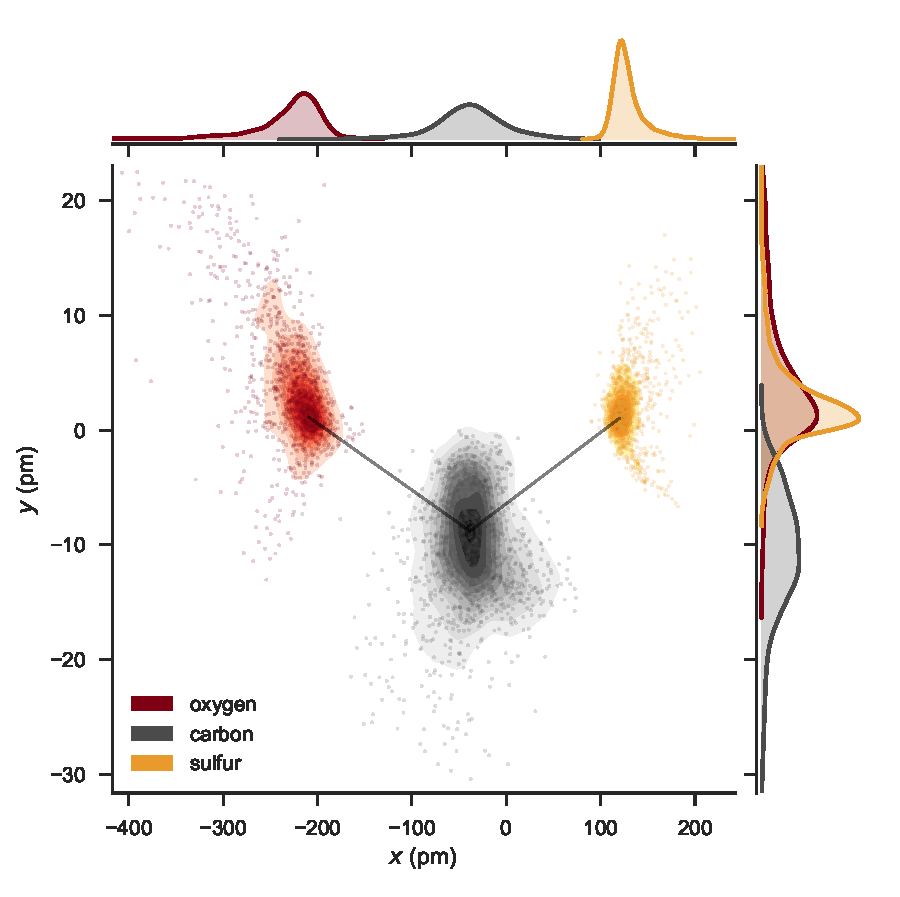
\includegraphics[width=\textwidth]{Plots/OCS2227fsMOGeometry}
  \caption[Scatter plot showing a reconstruction of the molecular geometry of \ch{OCS} following Coulomb explosion by a \SI{7}{\fs} laser pulse for the $(2,2,2)$ fragmentation channel.]
  {Scatter plot showing a reconstruction of the molecular geometry of \ch{OCS} following Coulomb explosion by a \SI{7}{\fs} laser pulse for the $(2,2,2)$ fragmentation channel. Each geometry is represented by three colored points, one for each atomic fragment; red for oxygen on the left, black for carbon in the center, and yellow for sulfur on the right. The colors were chosen to imitate the CPK coloring convention. Geometries are plotted such that the molecule's center of mass is at the origin to showcase the variance in each atomic fragment's position, and are rotated such that a vertical line bisects the \ch{O-C-S} bond angle. Bivariate kernel density estimates (KDE) with a Gaussian kernel, plotted as shaded-in contours, are used to estimate the the probability density of each atomic fragment's position (see section \ref{sec:kde} for a discussion of KDE's). Solid black lines are drawn between the peaks of each atomic fragment's kernel density estimate to illustrate the \emph{modal geometry} or most likely geometry. Along the top of the plot, univariate KDE's show the probability density of each atomic fragment's position along the $x$-axis, and the same is done for the $y$-axis along the right. The modal geometry is calculated to be $r_\mathrm{CO} = \SI{170}{\pico\m}$, $r_\mathrm{CS} = \SI{159}{\pm}$, $ \theta_\mathrm{OCS} = 173\degree$ while the average geometry of $r_\mathrm{CO} = \SI{193}{\pico\m}$, $r_\mathrm{CS} = \SI{168}{\pico\m}$, $ \theta_\mathrm{OCS} = 171\degree$ is slightly larger due to outliers. The molecule is almost straight but an aspect ratio of approximately $10:1$ is employed to showcase variability in the $y$-axis.}
  \label{fig:OCS2227fsMOGeometry}
\end{figure}

Before plotting, badly reconstructed geometries and duplicate geometries are filtered out. A badly reconstructed geometry satisfy at least one of three criteria. It (1) does not satisfy the KKT optimality conditions from section \ref{ssec:KKT} in which case the optimization algorithm is said to not have converged and \texttt{MultiStart} assigns such a geometry with an exit flag of $1$ making it easy to filter out such geometries. Or (2) it produces momentum vectors with a high absolute error when compared to the measured momentum vectors. We choose a threshold of $10^{-50}$ above which we say that the geometry is not precise enough to be a good reconstruction. The vast majority of reconstructions have significantly lower error ($10^{-59} - 10^{-54}$) and in general, geometries with a high absolute error do not satisfy (1) either. Or finally, (3) it lies very close to the box constraints (within $0.001$) that form our cuboid of physically realistic geometries in phase space. This usually indicates that the optimal geometry lies outside the constraints and that the solver asymptotically approached the boundary (due to the logarithmic barrier) in an attempt to converge on an optimal solution. Such bad geometries tend to also satisfy (1) and (2), but some redundancy is desirable to find all badly reconstructed geometries.

For our reconstruction, we configured \texttt{MultiStart} to use $50$ uniformly distributed starting points, which in hindsight was highly excessive. Out of $1,285$ sets of measured momentum vectors, we attempted to reconstruct each $50$ times, recovering $53,648$ geometries in total. $50,615$ represented duplicate geometries. Due to rounding errors involved with the comparison of floating-point numbers, we defined two triatomic geometries $i$ and $j$ to be duplicates if $\Delta_{ij} < 0.1$ where $\Delta_{ij} = |r_{12}^i - r_{12}^j| + |r_{23}^i - r_{23}^j| + |\theta^i - \theta^j|$ with bond lengths and angles being numerically described in picometers and degrees. After filtering out duplicate geometries, $3,033$ unique reconstructed geometries remain. $1,816$ had an exit flag of $1$ indicating a bad geometry (a non-optimal solution). No geometries with high error ($>10^{-50}$) were found, having all been previously found with an exit flag of 1. Then a further 91 geometries were found very close to the box constraints. Filtering out these $1,816 + 91 = 1,907$ bad geometries, we are left with $1,126$ ``good'' geometry reconstructions. $1,072$ were mapped to a single geometry, $18$ measurements to two distinct degenerate geometries, and $6$ to three distinct degenerate geometries. No measurement mapped to $4$ or more degenerate geometries, and $189$ measurements could not be reconstructed to satisfy our box constraints. In total, 2\% of measurements mapped to multiple degenerate geometries and $1,096$ measurements were successfully reconstructed, giving an 85\% success rate.

The recovered geometries are plotted in figure \ref{fig:OCS2227fsMOGeometry} and the geometries recovered for other laser pulse lengths (\SIlist{30;60;100}{\femto\s}) are plotted in appendix \ref{appx:supplementaryFigures} (figures \ref{fig:OCS22230fsMOGeometry}--\ref{fig:OCS222100fsMOGeometry}). The \SI{200}{\femto\s} data was not analyzed as the molecule seemed to have stretched too much for the lookup table reconstruction to seem trustworthy. Reconstruction statistics including success rate and number of degenerate geometries found for each pulse length is tabulated in table \ref{table:MOSuccess}. The modal and average geometries of for each pulse length are tabulated in table \ref{table:MOGeometries}.

% TODO: Discuss geometry plotting methods?

\begin{table}
  \myfloatalign
  \centering
  \begin{tabularx}{\textwidth}{cccc}
    \toprule
    Pulse length (\SI{}{\fs}) & Geometries & Reconstructions & Degenerate \\
    \midrule
    7 & 1285 & 1096 (85\%) & 18+6 (2.2\%) \\
    30 & 1501 & 1164 (76\%) & 62+30 (7.9\%) \\
    60 & 358 & 249 (70\%) & 15+6 (8.4\%) \\
    100 & 1056 & 694 (66\%) & 39+13 (7.5\%) \\
    \bottomrule
  \end{tabularx}
  \caption[Statistics for geometry reconstruction using constrained nonlinear optimization as a function of pulse length.]
  {Statistics for geometry reconstruction using constrained nonlinear optimization. The geometries column lists the number of experimental measurements (sets of momentum vectors) obtained, the reconstructions column lists the number and percentage of these measurements that were successfully reconstructed, and the degenerate column lists the number of measurements for which 2 and 3 degenerate geometries were found, respectively, and the percentage of successful reconstructions that yielded degenerate geometries. No measurement ever yielded more than 3 degenerate geometries.}
  \label{table:MOSuccess}
\end{table}

\begin{table}
  \myfloatalign
  \centering
  \begin{tabularx}{0.85\textwidth}{ccccccc}
    \toprule
    & \multicolumn{3}{c}{Modal geometry} & \multicolumn{3}{c}{Average geometry} \\
    Pulse length (fs) & $r_\mathrm{CO}$ & $r_\mathrm{CS}$ & $\theta_\mathrm{OCS}$ & $r_\mathrm{CO}$ & $r_\mathrm{CS}$ & $\theta_\mathrm{OCS}$ \\
    \midrule
    7 & 170 & 159 & 173 & 193 & 168 & 172 \\
    30 & 231 & 177 & 172 & 243 & 215 & 168 \\
    60 & 238 & 196 & 172 & 242 & 232 & 166 \\
    100 & 249 & 206 & 171 & 256 & 254 & 165 \\
    \bottomrule
  \end{tabularx}
  \caption[Average and modal geometries reconstructed using constrained nonlinear optimization as a function of pulse length.]
  {Average and modal geometries calculated from the geometries reconstructed using constrained nonlinear optimization as a function of pulse length. The bond lengths are given in picometers (\SI{e-12}{\m}) and the bond angles in degrees.}
  \label{table:MOGeometries}
\end{table}

% TODO: Discuss these tables.

\subsection{Comparision with the lookup table}
Comparing figures \ref{fig:OCS2227fsLTGeometry} and \ref{fig:OCS2227fsMOGeometry} we do not see much qualitative difference between the two. Figure \ref{fig:OCS2227fsMOGeometry} does have a greater number of reconstructions and data points. This is due to both the higher success rate (85\% versus 73\%) and since 500 more measurements were found since the lookup table was tested. Degenerate geometries contribute a small amount as well. The atomic positions exhibit greater variability in their positions, which may be because the optimization routine is able to reconstruct more extreme geometries than the lookup table could and with greater precision. The modal and average geometries calculated from both reconstructions are extremely similar.

While the overall geometry is not very different, the absolute errors on each geometry are much smaller. The lookup table produces geometries with absolute errors on the order of $10^{-48}$ at best due to its low resolution but the optimization routine finds geometries with errors on the order of $10^{-59} - 10^{-54}$, corresponding to an additional 3-5 decimal places of precision on the numerical values of the molecular parameters.

The optimization routine is also able to precisely find degenerate geometries by using multiple starting points, a task which would have been non-trivial for the lookup table.

\subsection{Investigating individual reconstructions} \label{ssec:weirdBonds}
Figure \ref{fig:OCS2227fsMOGeometry} provides an intuitive image of what a molecular geometry looks like, but it would be interesting to also see a distribution of bond lengths and bond angles to quantify the variability in each of these parameters. Correlations between the bond lengths and bond angles may also be looked at to study, for example, if longer \ch{C-O} bond lengths correspond to longer \ch{C-S} bond lengths, or if more bent geometries tend to have longer bond lengths. To visualize this relationship in figure \ref{fig:OCS2227fsMOGeometryPairs} we utilize a scatterplot matrix.

\begin{figure}
  \centering
  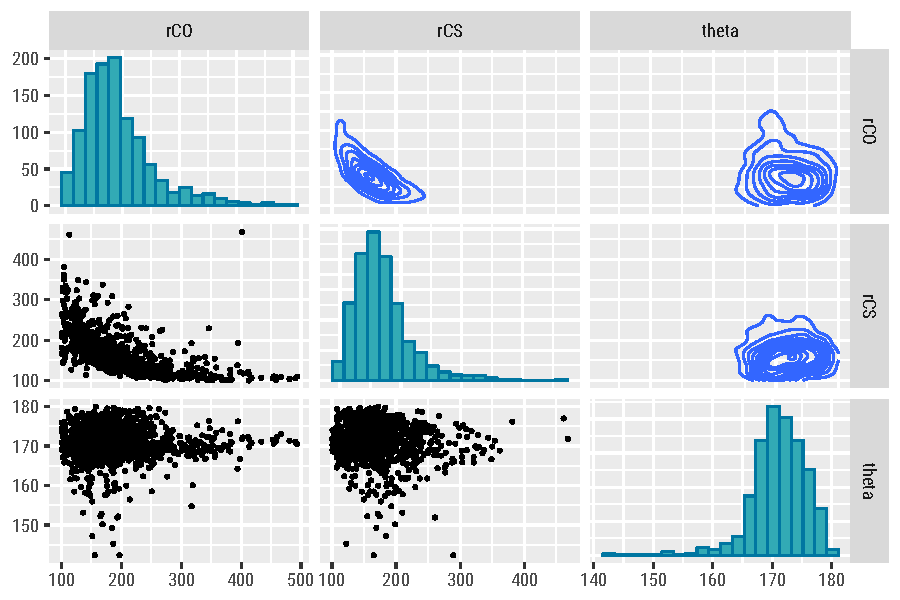
\includegraphics[width=\textwidth]{Plots/OCS2227fsMOGeometryPairs}
  \caption[Scatter plot matrix showing the bivariate relationship between the parameters $(r_\mathrm{CO}, r_\mathrm{CS}, \theta)$ for the reconstructions of the molecular geometry of \ch{OCS} following Coulomb explosion by a \SI{7}{\fs} laser pulse for the $(2,2,2)$ fragmentation channel.]
  {Scatter plot matrix showing the bivariate relationship between the parameters $(r_\mathrm{CO}, r_\mathrm{CS}, \theta)$ for the reconstructions of the molecular geometry of \ch{OCS} following Coulomb explosion by a \SI{7}{\fs} laser pulse for the $(2,2,2)$ fragmentation channel. On the diagonal, histograms show the distribution of bond lengths and bond angle for the reconstructed geometries (tick marks at the bottom of each column). Below the diagonal, scatter plots show the bivariate relationship between each molecular parameter. Above the diagonal, the same relationship is given using a contour plot instead.}
  \label{fig:OCS2227fsMOGeometryPairs}
\end{figure}

The bond length distributions on the diagonal of figure \ref{fig:OCS2227fsMomentum} are somewhat expected; they peak slightly above the equilibrium values indicating some molecular rearrangement and bond lengthening due to the molecule's interaction with the laser field. The bond angle distribution shows less variability suggesting that the molecule may have not had much time to bend yet, or that the laser's electric field primarily induces a lengthening in the bonds. This would seem expected as well, since the electric field's purpose is to quickly ionize the molecule which should cause the individual atoms to begin repelling each other as soon as the ionization occurs. % TODO: How similar is this to theoretical calculations?

What is very interesting, however, is the relationship between the two bond lengths, $r_\mathrm{CO}$ and $r_\mathrm{CS}$. We may intuitively expect both bond lengths to lengthen as the three atoms should repel each other in the $(2,2,2)$ charge state, or possibly to have one bond stretch while the other remains relatively constant. However, the reconstructions actually indicate the complete opposite---that while one bond stretches the other shrinks, almost following a reciprocal relationship. This effect becomes even more pronounced for reconstructions of molecular geometries exposed to longer pulse lengths (figures\ref{fig:OCS22230fsMOGeometryPairs} -- \ref{fig:OCS222100fsMOGeometryPairs}).

Such an unusual relationship suggests that our reconstruction efforts may have failed to account for a missing factor, or possibly that one of the assumptions we have made, particularly in simulating the Coulomb explosion (section \ref{sec:simulating}), is grossly invalid, or that some other part of our implementation requires revision. Unfortunately, to our knowledge no other studies performing geometry reconstruction using Coulomb explosion imaging have reported the correlations between their bond lengths and bond angles, so no comparisions or references can be made.\footnotemark~ When plotted, as in figure \ref{fig:OCS2227fsMOGeometry}, the geometries seem to be physically reasonable and so do the bond length and bond angle distributions on the diagonal of figure \ref{fig:OCS2227fsMOGeometryPairs}, it is only the correlations that do not. Analyzing the reconstructed geometries produced by the lookup table results in a very similar relationship between the bond lengths of reconstructed geometries.

\footnotetext{Private communication with collaborators suggests that other investigations have led to similar worrying results, leading to the abandonment of geometry reconstruction efforts.}

At this juncture, such worrying results force us to distrust the geometry reconstructions we have produced thus far. While the average geometries and overall dataset seems to be physically reasonable, the individual geometries seem to not make physical sense. Additionally, the same unusual relationship emerges out of at least two different reconstruction methods. For now we will move on to utilize the optimization routine to further investigate the nature of the degenerate geometries we are recovering, however we will come back and resolve this issue in the next chapter.

\section{Investigating degenerate geometries} \label{sec:optimizationDegeneracies}
The optimization approach should also be tested to study whether it can accurately reconstruct simulated geometries in the same manner we tested the Nelder-Mead simplex method (section \ref{ssec:simplexFail}) and the lookup table (section \ref{ssec:LTaccuracy}). We will also use this information to further investigate the nature of the degenerate geometries we are recovering.

The accuracy testing of the Nelder-Mead simplex method and the lookup table was relatively cursory, and could be made more thorough. We varied one molecular parameter at a time, which was however, sufficient to show the inadequecy of the simplex method. For a more thorough test, we will substantially vary all the molecular parameters by simulating the Coulomb explosion of geometries within a box in phase space described by $\SI{100}{\pico\meter} \le r_\mathrm{CO}, r_\mathrm{CS} \le \SI{500}{\pico\meter}$ and $\SI{140}{\degree} \le \theta \le \SI{180}{\degree}$. For a low-resolution test, we pick geometries $r_\mathrm{CO} \times r_\mathrm{CS} \times \theta_\mathrm{OCS}$ where $r_\mathrm{CO}$ and $r_\mathrm{CS}$ are sets containing $10$ uniformly spaced bond lengths between \SI{100}{\pico\meter} and \SI{500}{\pico\meter}, $\theta_\mathrm{OCS}$ is a set containing $10$ uniformly spaced bond angles between \SI{140}{\deg} and \SI{180}{\deg}, and $X \times Y = \lbrace (x,y) | x \in X \;\mathrm{and}\; y \in Y \rbrace$ denotes the cartesian product as expressed in set-builder notation \citep[p. 6]{Warner90}. Thus we are reconstructing $10^3 = 1,000$ geometries from simulated Coulomb explosions. We also perform a higher-resolution test using $20^3 = 8,000$ uniformly distributed geometries within the same box.

In both tests, we find that the optimization routine can reconstruct the simulated geometries in $98.5\%$ of cases using only a single starting guess. Each reconstruction takes approximately one second. In each of these reconstructions, the parameters of the recovered geometry numerically matched the original geometry up to several decimal places. The absolute error between the recovered and simulated momentum vectors was below $10^{-55}$ for $95\%$ of reconstructions, with the mean error being approximately $10^{-57}$, is 10 orders of magnitude lower than the absolute errors on momentum vectors retreived using the lookup table. Since we use the square of the $\ell_2$-norm to quantify the absolute error, this actually represents an improvement of approximately 5 orders of magnitude in accuracy over the lookup table. Using multiple starting points recovers geometries for the other $1.2\%$ of cases.

While the optimization routine recovered very precise geometries whose post-explosion momentum vectors very closely match the expected vectors, the geometries were not always the originally generated geometries which we expected. It seems that in about $5\%$ of cases, the routine returned a degenerate geometry. It is important to make the distinction that when the Nelder-Mead simplex method and the lookup table returned a different geometry than expected, it was a failure in recovering the exact geometry as the momentum vectors did not match closely resulting in a large absolute error (roughly $>10^{-46}$) (except for a small number of cases where it had found a degenerate geometry). However, in this case we are finding very precise reconstructions and each different geometry represents a degenerate geometry. To showcase the nature of these degenerate geometry, we plot arrows between the original (expected) geometry and the recovered degenerate geometry in figure \ref{fig:OCS222DegeneracyMaps}, which we will refer to as a \emph{degeneracy map}. If the recovered geometry was the original geometry as expected, then no arrow is plotted.

\begin{figure}
  \centering
  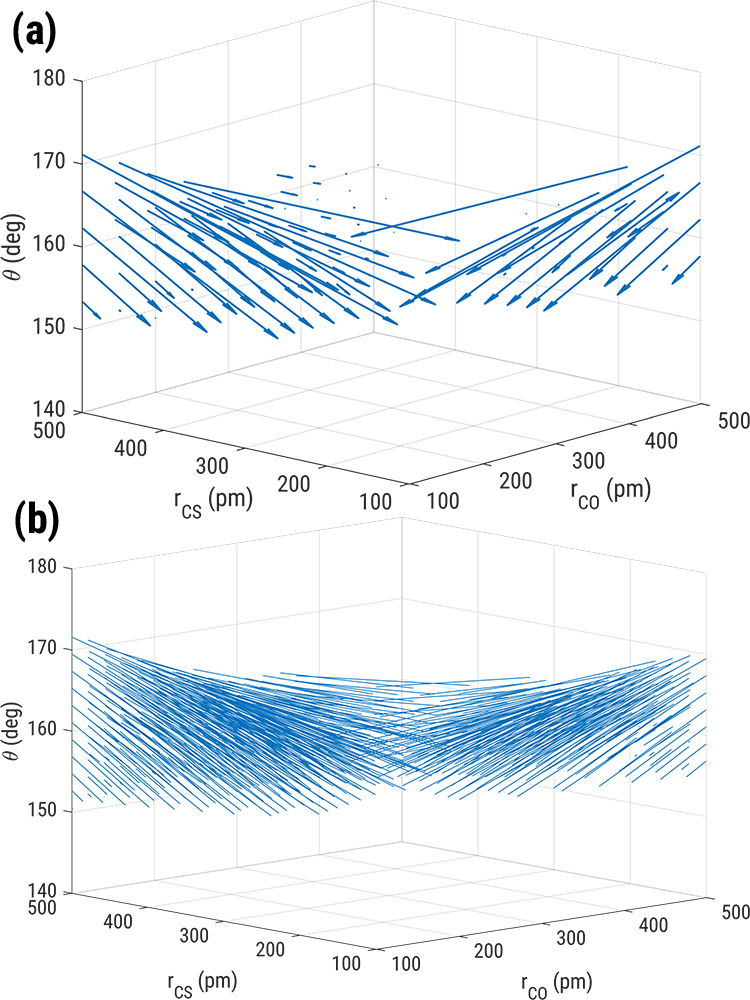
\includegraphics[width=\textwidth]{Plots/OCS222DegeneracyMap}
  \caption[Mapping between degenerate geometries for the \ch{OCS} $(2,2,2)$ molecule.]
  {Mapping between degenerate geometries for the \ch{OCS} $(2,2,2)$ molecule. The Coulomb explosion of (a) $1,000 \; (10^3)$ and (b) $8,000 \; (20^3)$ uniformly distributed geometries within a box in phase space described by $\SI{100}{\pico\meter} \le r_\mathrm{CO}, r_\mathrm{CS} \le \SI{500}{\pico\meter}$ and $\SI{140}{\degree} \le \theta \le \SI{180}{\degree}$ was simulated and then reconstructed using the momentum vectors of the atomic fragments that resulted from the simulations. If the reconstructed geometry matched the original geometry exactly, then no arrow is plotted. However, an (a) arrow or (b) line is plotted from the original expected geometry to the recovered geometry if it represented a degenerate geometry. Arrows and lines small enough that they resemble points indicate a slight numerical difference between the expected geometry and the reconstructed geometry, and do not neccessarily represent a degenerate geometry.}
  \label{fig:OCS222DegeneracyMaps}
\end{figure}

We see some patterns in the degenerate geometries recovered. Degenerate geometries exist only for molecules with bond angles between approximately \SI{150}{\deg} and \SI{170}{\deg} which includes a sizable minority of the molecules reconstructed as indicated by the bond angle distribution in figure \ref{fig:OCS2227fsMOGeometryPairs}. They also exist mainly for molecules exhibiting significant bond asymmetry and tend to be degenerate with another molecule that is more bent and has a smaller degree of bond length asymmetry. They also appear in two regions, one where the \ch{C-O} bond length is longer, and another where the \ch{C-S} bond length is longer. The discrete number of arrows figure \ref{fig:OCS222DegeneracyMapSD}(a) may suggest the existence of a discrete number of these degenerate geometries, however, repeating the test with a greater number of geometries produces very similar results except for a correspondingly higher density of lines, suggesting that regions exist in phase space where every geometry is degenerate with another, \ie~ that an uncountably infinite\footnotemark~ number of degenerate geometries exist.

\footnotetext{A countably finite set may refer to the set of integers $\mathbb{Z} = \lbrace 0, \pm 1, \pm 2, \dots \rbrace$, for example, which may be enumerated. An uncountably infinite set has the same cardinality as the set of real numbers $\mathbb{R}$ which cannot be enumerated \citep{Halmos17}.}

In these simulations we knew \textit{a priori} which geometry we expected to reconstruct, so we can assign a direction to each arrow. However, when reconstructing experimental data, we have no prior knowledge of what geometry we expected to recover, so the arrow could point in either direction. In some cases it might be possible to choose one degenerate geometry over the other(s) if one is physically unrealistic, \eg~ if it is very highly bent or exhibits an extreme bond length asymmetry.

\begin{figure}
  \centering
  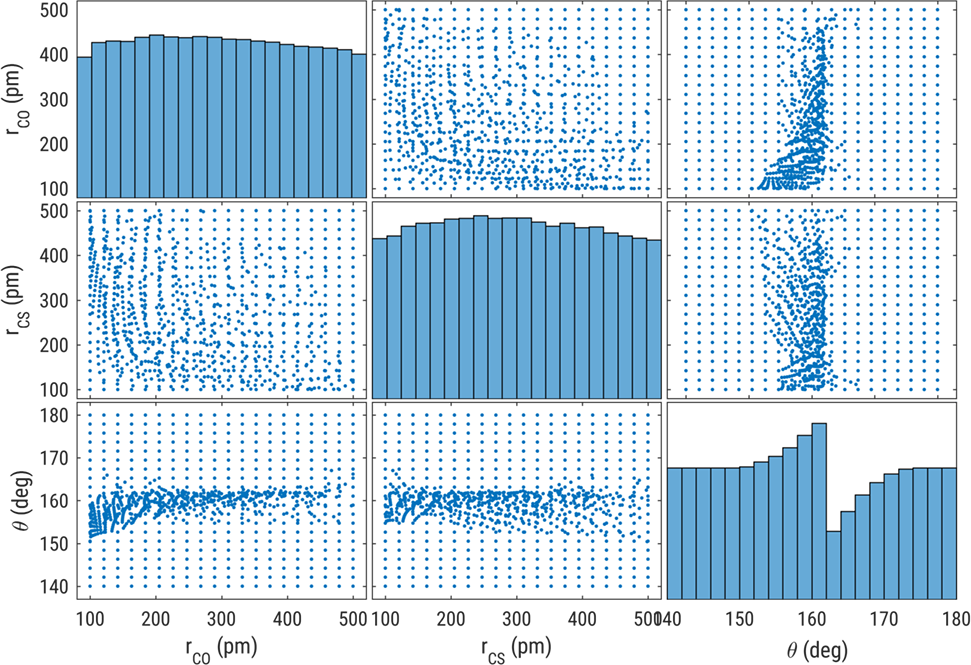
\includegraphics[width=\textwidth]{Plots/OCS222DegeneracyMapHDPairs}
  \caption[Scatter plot matrix showing the bivariate relationship between the parameters $(r_\mathrm{CO}, r_\mathrm{CS}, \theta)$ for the reconstructions of the molecular geometry of \ch{OCS} from momentum vectors obtained from simulated Coulomb explosions.]
  {Scatter plot matrix showing the bivariate relationship between the parameters $(r_\mathrm{CO}, r_\mathrm{CS}, \theta)$ for the reconstructions of the molecular geometry of \ch{OCS} from momentum vectors obtained from simulated Coulomb explosions of $8,000 \; (20^3)$ uniformly distributed geometries within a cuboid in phase space described by $\SI{100}{\pico\meter} \le r_\mathrm{CO}, r_\mathrm{CS} \le \SI{500}{\pico\meter}$ and $\SI{140}{\degree} \le \theta \le \SI{180}{\degree}$. On the diagonal, histograms show the distribution of bond lengths and bond angle for the reconstructed geometries with tick marks at the bottom of each column (no vertical scale is given for the histograms). Below the diagonal, scatter plots show the bivariate relationship between each molecular parameter. Above the diagonal, the same scatter plots are shown with the $x$ and $y$-axes interchanged to correspond with the axes labels and tickmarks.}
  \label{fig:OCS222DegeneracyMapHDPairs}
\end{figure}

To further visualize the set of geometries we recovered, we utilize a scatterplot matrix in figure \ref{fig:OCS222DegeneracyMapHDPairs} showing the bond length and angle distributions for the $8,000$ geometries used for accuracy testing as well as their bivariate relationships. It is interesting to note that whenever degenerate geometries exist, the more bent geometry is found. Perhaps these more bent solutions posess a larger \emph{basin of attraction}, which may or may not be strongly dependent on the optimization algorithm employed. It might be interesting to visualize them, possibly taking a similar approach as \citet{Asenjo13} who actually employ mathematical optimization methods to determine energy minimizing molecular structures. They observe basins with rather complicated boundaries, reminiscent of the beautiful and spatially chaotic patterns produced by the magnetic pendulum.

For the feasibility of geometry reconstruction, however, this result raises additional issues past the unusual bond length correlations found in the previous section. Even when the measured momentum vectors can be mapped to a molecular geometry very precisely, the existance of multiple solutions corresponding to very different geometries may make it impossible to perform accurate geometry reconstructions, especially when multiple degenerate geometries represent physically realizable geometries. Table \ref{table:lookupTableSuccess} also suggests the existence of triply degenerate geometries, which may further complicate the task of geometry reconstruction.

Interestingly, we find that we recover degenerate geometries approximately $5\%$ of the time while \citet[supplementary information]{Kunitski15} report finding degenerate geometries approximately $10\%$ of the time, although they chose to disregard them for their analyses.

We considered whether these degeneracies could arise due to our choice of momentum convention in section \ref{sec:conventions} however our convention simply rotates the three momentum vectors such that the carbon's momentum vector lies along the $+x$-axis and all three momentum vectors lie in a plane. The length of the momentum vectors and the relative angles between them remain unchanged, and so two different geometries producing different momentum vectors cannot result in the same set of vectors after rotation into our convention, unless they represent degenerate geometries.

\section{Conclusions}
\emph{Geometries may be reconstructed quickly and precisely using constrained nonlinear optimization}---This approach represents a significant improvement over the geometry reconstructions provided by the lookup table. Reconstructing a single geometry can be done in approximately one second, which is faster than the lookup table if enhanced precision is desired. Furthermore, the recovered molecular parameters are orders of magnitude more precise than those provided by the lookup table, and degenerate geometries may be found precisely.

%\subsection{Lessons learnt}
%\emph{Individual reconstructed geometries must be investigated}--- \\
%
%\noindent
%\emph{Regions in phase space containing degenerate geometries make geometry reconstruction more difficult}--- 
%
%\subsection{Future directions}
%\emph{Reconstruction of larger molecules}--- \\
%
%\noindent
%\emph{More efficient optimization}---